\section{MODELO DIMENSIONAL}
El modelo multidimensional dentro del entorno de las bases de datos, es una disciplina de diseño que se sustenta en el modelo entidad-relación y en las realidades de la ingeniería de texto y datos numéricos.\\\\ 
Modela las particularidades de los procesos que  ocurren en una organización, dividiéndolos en mediciones y entorno. La medidas son en su mayoría, medidas numéricas, y se les denomina hechos. Alrededor de estos hechos existe un contexto que describe en qué condiciones y en qué momento se registró este hecho. Aunque el entorno se ve como un todo, existen registros lógicos de diferentes características que describen un hecho, por ejemplo, si el hecho referido, es la venta de un producto en una cadena de tiendas, se podría dividir el entorno que rodea al hecho de la cantidad vendida, en el producto vendido, el cliente que lo compró, la tienda y la fecha en que se realizó la venta. A estas divisiones se le denomina dimensiones y a diferencia de los hechos que son numéricos, estos son fundamentalmente textos descriptivos.\\\\ 
Las medidas, como se  expresó anteriormente, se registran en las tablas de hechos, siendo la llave de esta tabla, la combinación de las múltiples llaves foráneas que hacen referencia   a las dimensiones que describen la ocurrencia de este hecho, en otras palabras, cada una de las llaves extranjeras en las tablas de hecho se corresponden con la llave primaria de una dimensión.\\\\ 
Esta técnica goza de una gran aceptación y, a menudo, es elegida como la preferida para representar datos analíticos por cumplir simultáneamente con los siguientes requerimientos:\\\\ 
Dispone y estructura los datos de manera comprensibles para el usuario de negocio\\
Genera un alto rendimiento en las búsquedas desde la capa de reporting\\
Dentro del modelado de datos dimensional destacan 2 conceptos clave: hechos y dimensiones.\\\\
\textbf{Hechos:} Son las métricas, normalmente valores cuantitativos (numéricos) susceptibles de ser agregados\\
Ejemplo: La cantidad de ventas de coches de un concesionario, el rendimiento en euros de una empresa, el número de estudiantes de un colegio, etc.\\\\
\textbf{Dimensiones:} Son los valores cualitativos. Proporcionan descripciones a los hechos, aportando un contexto a los mismos.\\
Ejemplo: Marca de coche, fecha, nombre concesionario, dirección de la empresa, nombre del colegio, etc.\\\\
Existen 2 técnicas para llevar acabo el modelado dimensional: el esquema de estrella y el esquema de copo de nieve.\\\\

\section{ESQUEMA DE ESTRELLA}

Un esquema de estrella es un modelo de datos formado por una tabla de hechos, que contiene los datos para el análisis, rodeada de las tablas de dimensiones.\\\\

\begin{center}
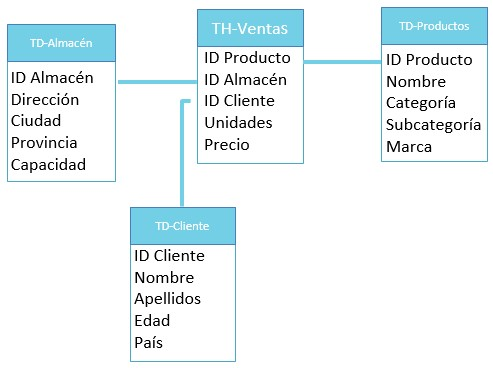
\includegraphics[width=12cm]{./Imagenes/imag1}
\end{center}

Como podemos observar en la imagen 1 la tabla de hechos es TH-Ventas y está rodeada de las dimensiones TD-Almacén, TD-Producto y TD-Cliente, almacenando el ID de cada dimensión en la tabla de Hechos para, así, poder relacionar los atributos descriptivos de cada dimensión con la fila de la tabla de hechos.\\\\
El modelo estrella separa los datos del proceso de negocio en: hechos y dimensiones. Los hechos contienen datos medibles, cuantitativos, y las dimensiones los atributos que describen los datos indicados en los hechos.\\\\
\textbf{TABLA DE HECHOS}\\\\
-Clave principal compuesta por los claves principales de las tablas de dimensiones\\\\
-Registra medidas o métricas de un evento específico. Ejemplo: cliente compra un geranio de maceta de 25cm en floristería mineral vegetal Lola a las 12:3 0am del 10 de Octubre de 2027\\\\
-Evita repetir de manera completa los atributos dimensionales. En la TH sólo irá un ID de la dimensión\\\\
-Se diseñan según el nivel de granularidad deseado, pudiendo registrar eventos a un gran nivel de atomicidad\\\\
\textbf{TABLA DE DIMENSIONES}\\\\
Tienen una clave primaria simple.\\\\
-Generalmente tienen un número bajo de registros\\\\
-Cada registro puede contener un gran número de atributos\\\\
-Suelen contener una surrogate primary key, generalmente una columna de tipo entero\\\\
\textbf{Las principales ventajas del esquema de estrella son:}\\\\
-Queries simples. Las uniones y cruces son más sencillos, debido a su lógica, que los de un esquema normalizado\\\\
-Lógica de reporting simplificada\\\\
Mejoras en el rendimiento de las consultas\\\\
-Agregaciones más rápidas. Gracias a las queries simplificadas\\\\
\textbf{Las principales desventajas del esquema de estrella son:}\\\\
-Poco flexible. Los esquemas en estrella son construidos para una vista de los datos en particular.\\\\

\section{ESQUEMA EN COPO DE NIEVE}\\\\

Un esquema de copo de nieve es una estructura más compleja que el esquema de estrella. Se da cuando alguna de las dimensiones se implementa con más de una tabla de datos.\\\\
El objetivo es normalizar estas tablas y reducir el espacio de almacenamiento al eliminar la redundancia.\\\\
Se representa como una tabla de hechos conectada con dimensiones anidadas. Al normalizar por completo las dimensiones el resultado parece un copo de nieve.\\

\begin{center}
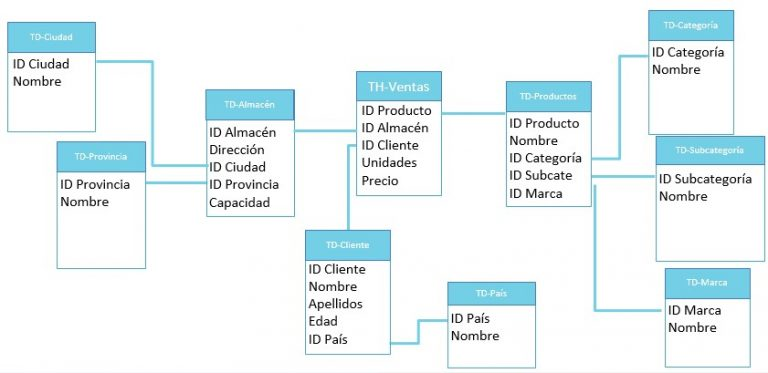
\includegraphics[width=15cm]{./Imagenes/imag2}
\end{center}
Observamos en la imagen 2 como se dividen las dimensiones de TD-Almacén, TD-Producto y TD-Cliente en sub-dimensiones normalizadas.\\\\
\textbf{Las principales ventajas del esquema de copo de nieve son:}\\\\
-Algunas herramientas de modelado de bases de datos multidimensional OLAP se optimizan\\\\
-La normalización de los atributos reduce el almacenamiento de datos\\\\
\textbf{Las principales desventajas del esquema de copo de nieve son:}\\\\
-Queries complejas debido a la normalización (implica un mayor número de cruces)\\\\
-Bajo rendimiento debido a la normalización\\\\
\section{CICLO DE VIDA DEL MODELO DIMENSIONAL}\\
En la vida de un modelo dimensional existen cuatro fases clave:\\\\
\textbf{Diseño:} puede utilizar el entorno de trabajo para crear modelos dimensionales.\\\\
\textbf{Prueba:} puede utilizar el entorno de trabajo y otras herramientas de consulta para analizar y probar un modelo dimensional en una base de datos (generalmente una base de datos de prueba).\\\\
\textbf{Transformación:} puede transformar los modelos de datos para trabajar con otras herramientas de consulta o para continuar desarrollando los modelos de datos y las aplicaciones.\\\\
\textbf{Producción:} es la fase de despliegue del modelo dimensional, y los usuarios pueden realizar consultas en la base de datos.


% Bibliografía.
%-----------------------------------------------------------------
\begin{thebibliography}{99}
https://blog.bi-geek.com/modelo-dimensional/\\
https://www.ibm.com/support/knowledgecenter/es/SS9UM9_9.1.2/com.ibm.datatools.dimensional.ui.doc/topics/c_dm_lifecycle.html\\
https://www.ibm.com/support/knowledgecenter/es/SSGU8G_11.50.0/com.ibm.ddi.doc/ids_ddi_350.htm\\
•	Á1.  ALBANO, A., ROSA, L. D., DUMITRESCU, C., GOGLIA, L., GOGLIA, R.  AND MINEI, V. Another Example of a Data Warehouse System Based on Transposed Files. En 10th International Conference on Advances in Database Technology: Springer-Verlag, 2006, p. 1110-1114. 2.\\
•	BOATENG, O., SINGH, J., GREESHMA AND SINGH, P. DATA WAREHOUSING. Business Intelligence Journal, 2012, vol. 5 (no. 2), pp. 224-234. 3. \\
•	STONEBRAKER, M., ABADI, D. J., BATKIN, A. AND CHEN, X.  C-Store: A Column-oriented DBMS En 31st Very Large Data Bases (VLDB) Conference, Trondheim, Norway, 2005. 4.\\
•	RUSSO, M., FERRARI, A.  AND WEBB, C. Microsoft SQL Server 2012 Analysis Services: The BISM Tabular Model. Microsoft Press, 2012. 5.\\ 
•	GARCÍA, L., SIMÓN, A., TORRES, M. AND ESPINOSA, Y. Solución de inteligencia de negocios para la integración de la información comercial y contable.  En Congreso Internacional de Matemática y Computación 2013, La Habana, Cuba, 2013. 6.  EVELSON, B. AND NICOLSON, N. Topic Overview: Business Intelligence.  2008. Disponible en Internet:<http://bit.ly/foresterbi>.  7.  BERNABEU, R. D. HEFESTO. Data Warehousing: Investigación y Sistematización de Conceptos. Hefesto: Metodología para la Construcción de un Data Warehouse. Córdoba, Argentina, 2010. 8.\\  


\bibitem{Cd94} Autor, \emph{Título}, Revista/Editor, (año)

\end{thebibliography}

\end{document}

